\documentclass[12pt]{article}
\usepackage[a4paper, bindingoffset=0.2in, %
							left=0.5in,right=0.5in,top=0.5in,bottom=0.5in,%
							footskip=.25in]{geometry}
\usepackage{graphicx}
\usepackage{listings}
\usepackage{amssymb}
\usepackage{hyperref}

\title{PSet1 Report}
\author{Ali Abolhassanzadeh Mahani}
\date{Sep. 28}

\begin{document}
    \maketitle
    \section{Problem 1}
    \subsection{Creations and the loops}
    For starters, since I know how many steps I'm going to have and the size of the row,
    I allocate a table of that size in memory using \texttt{np.ndarray} with \texttt{int} as my data type; This will be my canvas.
    
    Now,  I do a nested for loop for each \textit{round} and each \textit{element} in the row
    to find their situation and decide their next state. Here, some people use 
    \texttt{(index) \% len(row)} to set the boundary condition, but with this setup, we are doing a \texttt{mod operation} per element and it makes it a little inefficient. I used the fact that Python \texttt{ndarray}s support \emph{negative indexing} and just set the upper boundary condition with an if statement.
    
    \subsection{The rule}
    Our rule is as follows: \emph{``If \underline{only one} of my neighbors is 1 (i.e. Has a hat), I become 1 (i.e. put on the hat), otherwise, I become 0."}
    
    The mathematical interpretation of \emph{``If only 1 neighbor is 1"} is that the sum of the neighbors equals to 1. Hence the \texttt{if} statement in our code.
    
    \subsection{Fancy}
    The style of which I have written this code is to be able to import the functions, if I
    need them in the future. All that the last \texttt{if} statement does, is to see if we are executing this file, and then, execute the \texttt{main()} function.
    
    \subsection{Analysis}
    The main part of the code is the \texttt{put\_hat()} function, which consists mainly of two
    nested \texttt{for} loops. taking one to have $m$ iterations and the other, $n$, we can see 
    that the runtime complexity of this code is $\mathcal{O}(m.n)$.
    In order to analyze this code, one can run a profiler on it as follows:
    \begin{lstlisting}[language=bash]
    	python -m cProfile -s time Hats.py
    \end{lstlisting}
	Note that this profiler lists all the modules that are being called, so due to our use of \texttt{numpy} and \texttt{matplotlib.pyplot}, it will show a lot of things, but the main 
	function \texttt{put\_hats} will be at the top few.
    
	
	\subsection{Results}
	I used the \texttt{pcolormesh()} module from the \texttt{matplotlib.pyplot} library to
	export my canvas into a file. The resulting image is identical to rule 18, 26 or 90. (Figure \ref{fig:hats200})
	\begin{figure}[h!]
		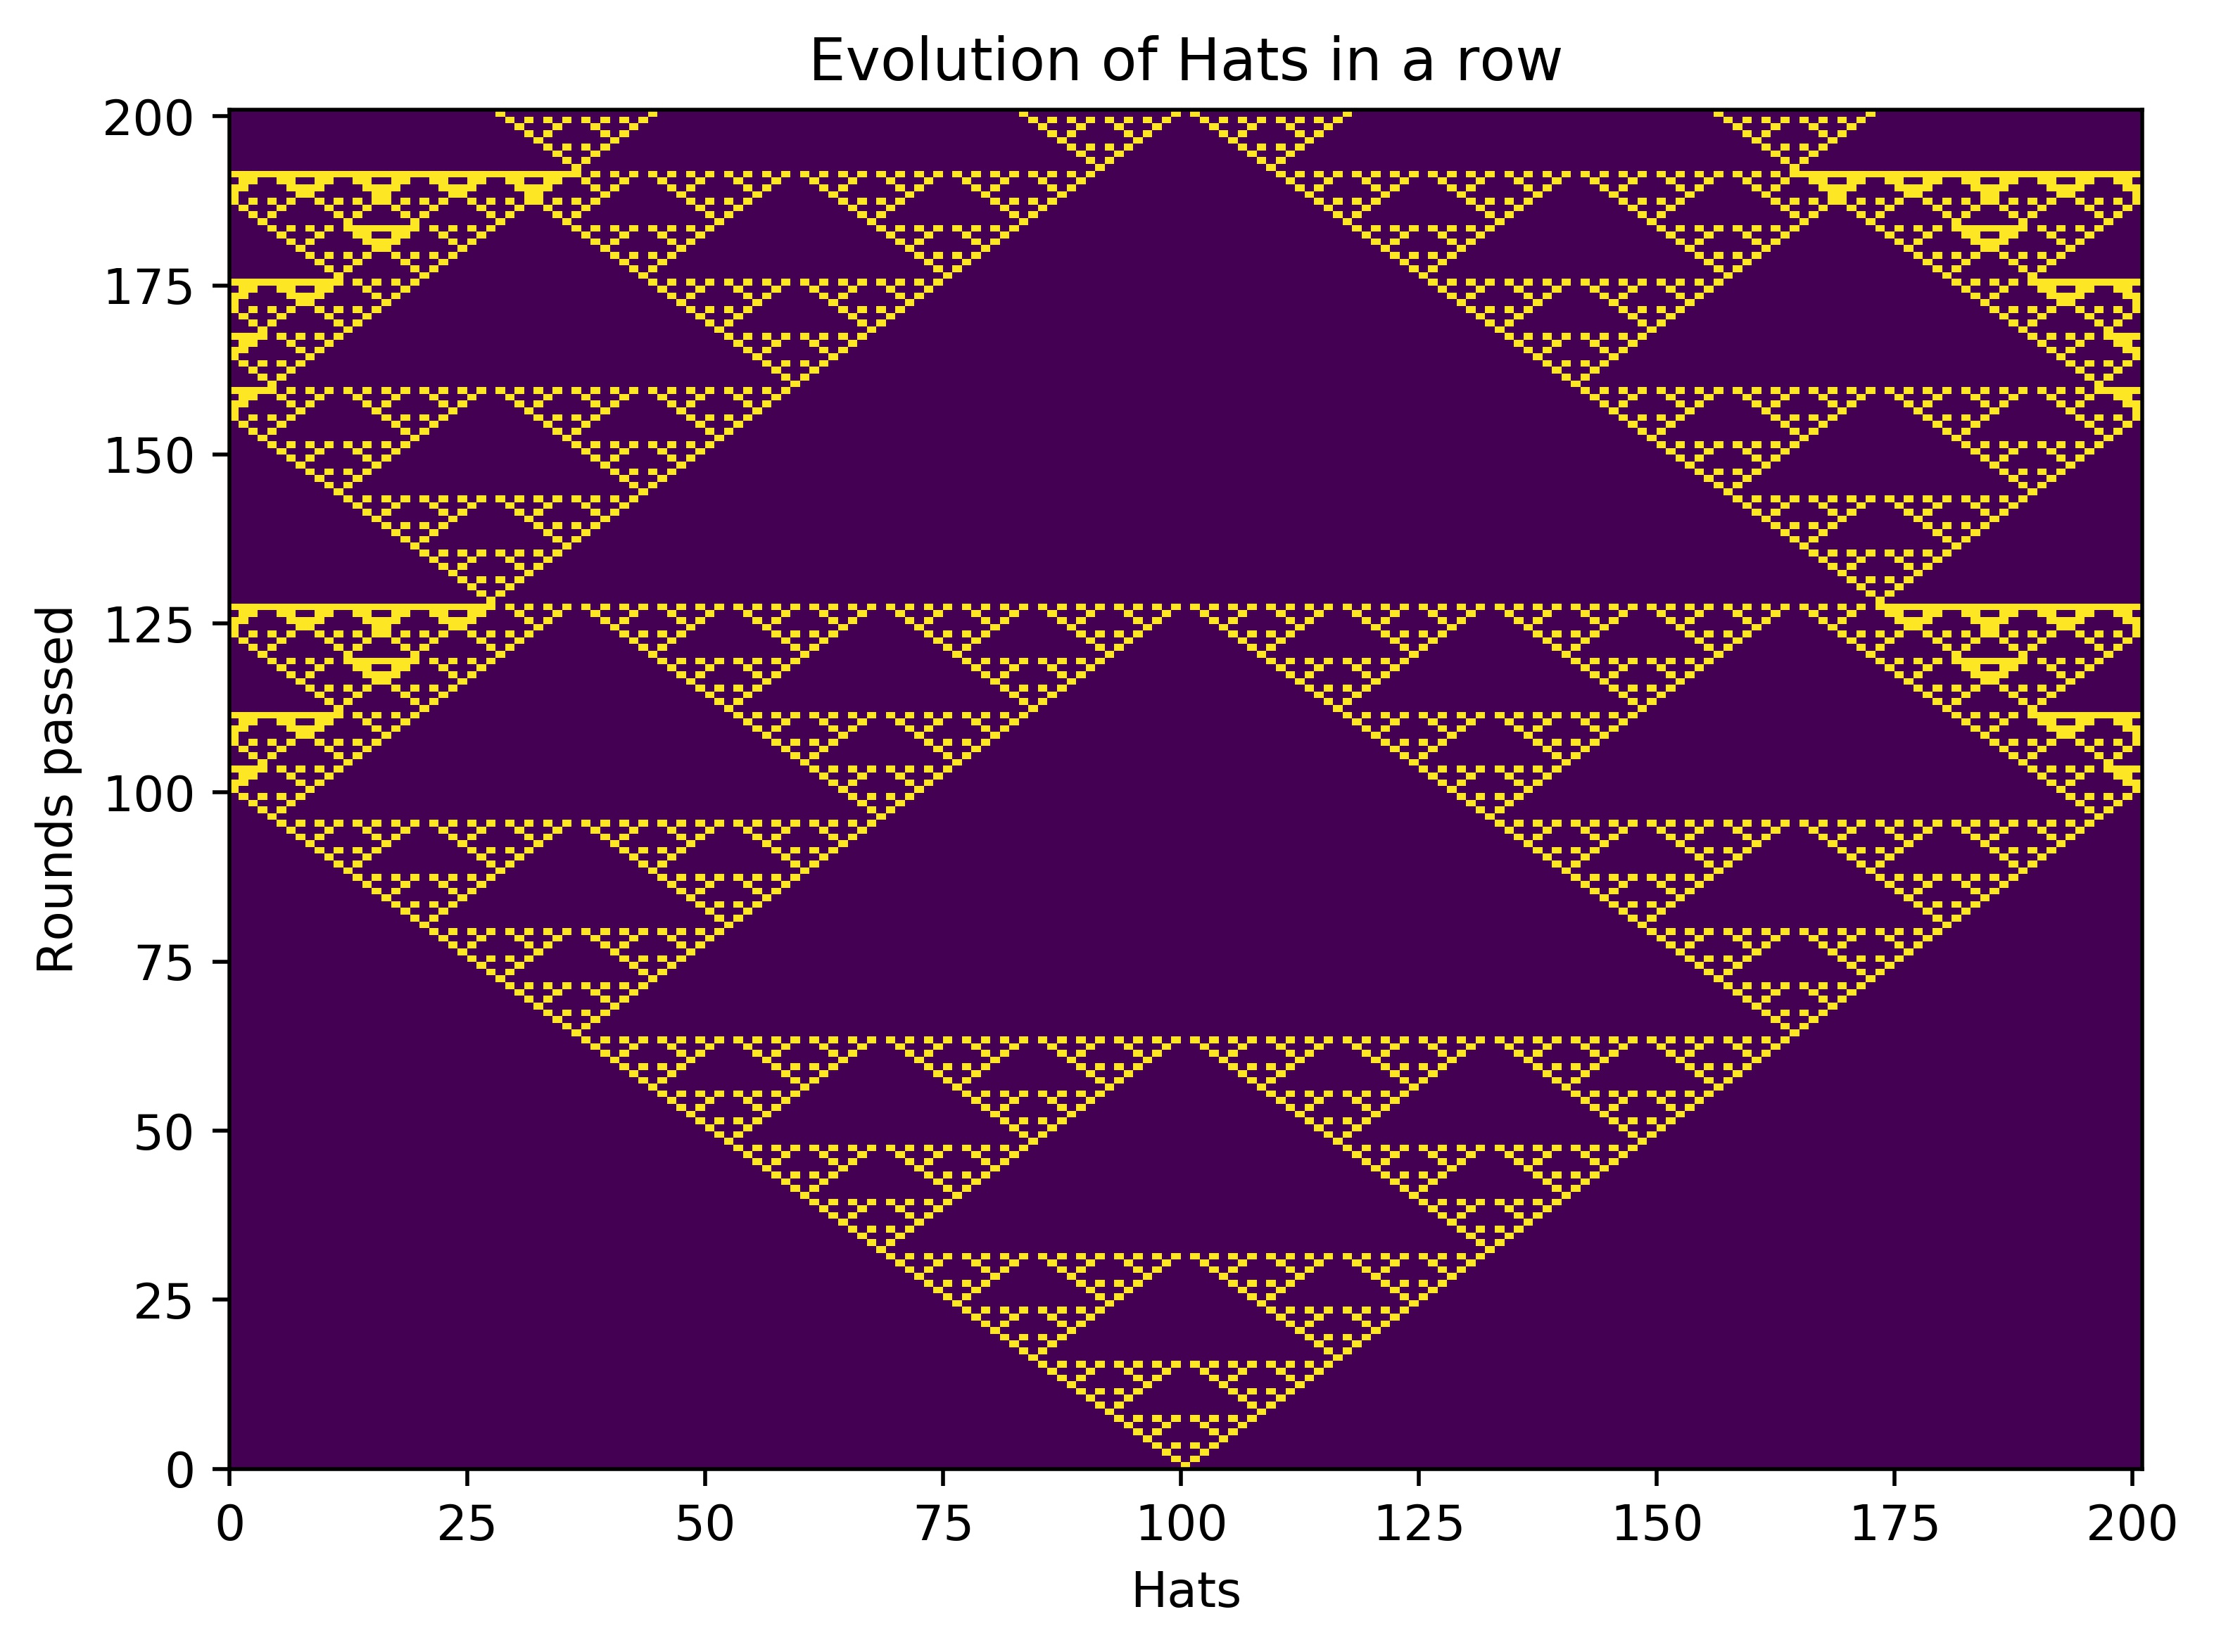
\includegraphics[width=\linewidth]{../P1/Hats200.jpg}
		\label{fig:hats200}
		\caption{The evolution of the hats for 200 steps using the rule that if only one of
							my neighbors has a hat, I put on a hat, otherwise, I put down my hat. The yellow cells have a hat on and the purple ones don't.
							\emph{Note that this rule is independent of the item in question.}}
	\end{figure}

	
	
\end{document}
